\section{Formular}\label{Formular}
Dieses Kapitel beschäftigt sich mit der Verwendung von Formularen in Wordpress.Dazu wird neben dem Begriff eines Formulars auch auf Beispiele aus der Mentoren-Suche zurückgegriffen. 
\subsection{Was ist ein Formular?}
Um überhaupt Formulare in Wordpress entwickeln zu können, soll an dieser Stelle zuerst eine Definition erwähnt werden. \newline
Laut SelfPHP\footcitetint[Vgl.][]{SEPHFP13} handelt es sich bei einem Formular um eine Maske, in der ein Benutzer Daten eingeben kann. Diese werden dann von einem Server verarbeitet und wenn erforderlich zurückgegeben. Dabei wird das Formular mittels dem HTML-Tag \emph{form} realisiert. Dabei kommen die beiden HTML-Methoden POST (vgl. Abschnitt \ref{post}) und GET (vgl. Abschnitt \ref{get}) zum Einsatz. 
Diese werden nun erläutert.
\subsubsection{POST-Methode}\label{post}
Einer der beiden Methoden\footcitetint[Vgl.][]{SEPHFP13}, um mit Formularen zu arbeiten, ist die POST-Methode. Diese wird dann eingesetzt, wenn ein Client eine Anforderung an einen Server sendet, dass weitere Daten übertragen werden sollen. Dabei sollte beachtet werden, dass die gesendeten Daten Teil von der vom Server festgelegten \gls{URI} ist.\newline
Der Zweck von POST liegt darin, Formulardaten an den Server zu übertragen. 
\subsubsection{GET-Methode}\label{get}
Hingegen zur POST-Methode ist die GET-Methode\footcitetint[Vgl.][]{SEPHFP13} dafür da, alle möglichen Informationen mittels der Ergebnis-\gls{URI} zu identifizieren. Eine komplette \gls{URI} besteht demnach aus 4 Bestandteilen:
\begin{enumerate}
	\item Die \gls{URI}
	\item Die \gls{URL}
	\item Einem Fragezeichen, welches als Trennzeichen verwendet wird
	\item Den gesendeten Daten
\end{enumerate}
Insgesamt lässt sich feststellen, dass POST-Methode die gesendeten Daten im Body (adressiert durch Header) sendet, während die GET-Methode diese als Teil der \gls{URL} betrachtet und mit anhängt.\newline
Abschließend lässt sich formulieren, dass für das Plugin Mentoren-Suche die Post-Methode verwendet wurde, da es sich um vertrauenswürdige Daten handelt und diese durch GET manipulierbar wären - genauer gesagt durch die Manipulation der \gls{URL}. Aus diesem Grunde wird in den folgenden Beispielen auch nur die POST- und Wordpress-Methode angesprochen. Der zweiten wird sich im nächsten Abschnitten gewidmet.
\subsection{Wordpress-Formulare}\label{wpform}
Auch Wordpress bietet eine Methode an, um mit Formularen zu arbeiten. Es handelt sich hierbei um eine vordefinierte Action von Wordpress, um beispielsweise Mentoren mit Vor- und Nachname sowie einem Bild und E-Mail-Adresse einzutragen.\footcitetint[Vgl.][]{MMTFRDA13} \newline 
Die genauere Syntax ist in der folgenden Aufzählung dargestellt.
\begin{enumerate}
	\item \textbf{do\_action}
	\begin{itemize}
		\item Führt einen Hook aus, der mittels add\_action (vgl. Abschnitt \ref{refmitaddacunaddfilt}) erstellt wurde.
		\item Die Syntax ist folgendermaßen definiert
		\begin{itemize}
			\item do\_action( \$tag, \$ arg);
			\begin{itemize}
				\item \$tag beschreibt des auszuführenden Hook und muss angegeben werden.
				\item \$arg Beschreibt einen optionalen Parameter, welcher eine Liste von anzugebenen Argumenten für den Hook darstellt.
			\end{itemize}
		\end{itemize}
	\end{itemize}	
\end{enumerate}
Nachdem die beiden grundlegenden Techniken besprochen wurden, werden im nächsten Kapitel die Theorie mit der Praxis angereichert und Beispiele erläutert. 
\subsection{Beispiel Formular aus Mentoren-Suche}
An dieser Stelle werden nun Beispiele für Formulare aus der Mentoren-Suche gezeigt und erläutert.\newline
Dabei wird zuerst ein Beispiel für ein PHP-Formular und abschließend die Wordpress-Methode vorgestellt.
\subsubsection{Beispiel für PHP-Formular}
In diesem Unterkapitel geht es um ein PHP-Beispiel, welches in Listing \ref{BSPFORMINWP} dargestellt ist.
\lstset{language={PHP},caption={Beispiel Formular in Wordpress},label=BSPFORMINWP}
\lstset{
 morekeywords={function,do_action,global,\$exit_msg}
}
\begin{lstlisting}
function ms_getOptionsPage()
{
echo "<h2>".__('Frontend-Seiten:','mentoren-suche')."</h2>";
echo "<p>".__('ANLEITUNG ZUR BENUTZUNG.','mentoren-suche')."</p>";
echo "<form action=\" \" method=\"post\">
  <table>
			<tr>
       		    	//Suchformular
			</tr>
  </table>
   		 
    <tr>
     <td colspan=\"2\"><input type=\"submit\" 
     name=\"ms_options_save\" 
     value=\"".__('Speichern','mentoren-suche')."\">
     </td>
    </tr>  
                     
  </table>
</form>";   
    
if(isset($_POST['ms_options_save']))
  {
    ms_options_update();
    echo "<h2 class=\"ms_info_message\">".
         __('Bitte aktualisieren Sie die Browseransicht (z.B. 
            mit F5), um die ver&auml;nderten Daten zu 
            sehen.','mentoren-suche')."</h2>"; 
  }
 }
}
\end{lstlisting}
Dieses Beispielformular aus Listing \ref{BSPFORMINWP} ist in verkürzter Art und Weise dargestellt, würde aber insgesamt wie in Abbildung \ref{img:BSPFORM} aussehen.
  \begin{figure}[htbp]
	\begin{center}
	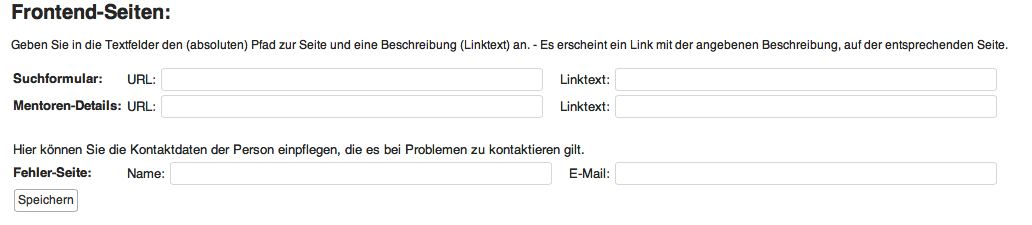
\includegraphics[angle={360}, scale=0.45]{pictures/form.png}
	    \caption{Beispielformular mittels PHP}
	    \label{img:BSPFORM}
	\end{center}
   \end{figure}
   \ \newline
Der Zweck dieses Formulars ist es, Einstellungen für das Plugin vorzunehmen. Dies geschieht in Form von Textfeldern, welche entsprechend ausgefüllt werden müssen.\newline
Erkennen lassen sich in Zeile 5 und Zeile 22 - 29 die POST-Methode. \newline
Nachdem die einzelnen Daten in die dafür vorgesehenen Felder eingetragen und der Speicher-Button aktiviert (\emph{ms\_options\_save}) wurde, wird in Zeile 22 die Funktion \emph{ms\_options\_update} aufgerufen. Der Zweck hinter dieser Funktion liegt darin, die Einstellungen für die Daten des geänderten Mentoren oder Mentees zu ändern.\newline
So würde ein Beispiel für eine Post-Methode in der Mentoren-Suche aussehen. Weitere Informationen zu dem Thema finden sich unter:
\begin{itemize}
	\item \url{http://www.selfphp.info/praxisbuch/index.php}
	\item \url{http://www.phpbox.de/php\_tutorials/formularversenden1.php}
\end{itemize}
\subsubsection{Beispiel für Wordpress-Formular}
Nachdem ein Beispiel mit der POST-Methode gezeigt und erläutert wurde, wird nun die Wordpress-Variante behandelt.\newline
Wie schon angesprochen, wird bei dieser Art die do\_action-Anweisung verwendet (vgl. \ref{wpform}). Diese ist beispielhaft in Listing \ref{BSPFORMINWP} dargestellt.
\lstset{language={PHP},caption={Beispiel Formular in Wordpress},label=BSPFORMINWP}
\lstset{
 morekeywords={function,do_action,global,\$exit_msg}
}
\begin{lstlisting}
function ms_row_new() {
	
	global $wpdb;
	global $title;
	echo "<h1>".$title."</h1>";
	
	echo "<div id=\"ms_row_new\">  
        <div class=\"register-form\">  
        <div class=\"title\">  ".
           "<h3>".__('Mentor eintragen','mentoren-suche')."</h3>
        </div>  
        <form
           //Formular

		  do_action('ms_insert_mentor');
			
		  echo " <input type=\"submit\" value=\"Eintragen\" id=\"register\" />  
		  
        </form>  
	</div>
</div>  ";

...
?>
\end{lstlisting}
Die in Listing \ref{BSPFORMINWP} dargestellte Funktion hat den Zweck, die Oberfläche für "Datensatz eintragen" funktional darzustellen. Dies ist in Abbildung \ref{img:BSPFORMWP} bildhaft dargestellt.
  \begin{figure}[htbp]
	\begin{center}
	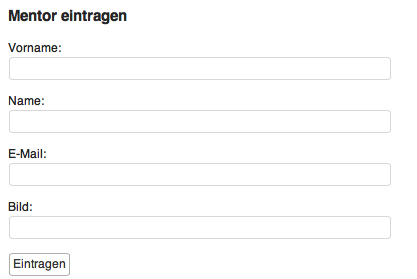
\includegraphics[angle={360}, scale=0.46]{pictures/formwp.png}
	    \caption{Beispielformular mittels do\_action}
	    \label{img:BSPFORMWP}
	\end{center}
   \end{figure}\ \newline
Was sich direkt erkennen lässt, sind die beiden Form-Tags in den Zeilen 12 und 19. Dazwischen befindet sich zum einen das Formular, zum anderen aber auch ein Button (\emph{Eintragen}) zum Bestätigen der Eingabe und ich Zeile 15 die \emph{do\_action}-Anweisung.\newline
Was hier nun passiert ist einfach zu erklären: Mittels der \emph{do\_action}-Anweisung wird die Action \emph{ms\_insert\_mentor} aufgerufen. Diese wiederum ruft in der Hauptdatei \emph{mentoren\_suche.php} die Action ms\_m\_data\_insert auf (siehe Listing \ref{AUACDDOACANW}).
\lstset{language={PHP},caption={Ausgeführte Action der do\_action-Anweisung},label=AUACDDOACANW}
\lstset{
 morekeywords={function,do_action,global,\$exit_msg}
}
\begin{lstlisting}
<?php
...
add_action('ms_insert_mentor','ms_m_data_insert');
...
<?
\end{lstlisting}
Diese wiederum ist dafür verantwortlich, nach dem Bestätigen des Submit-Buttons aus der Zeile 17 des Listing \ref{BSPFORMINWP}, die angegebenen Mentoren in die Mentorentabelle der Datenbank einzutragen.\newline
Vollständigerweise ist diese Funktion in Listing \ref{AUFGERACT} dargestellt und wird anschließend kurz erläutert.
\lstset{language={PHP},caption={Aufgerufene Funktion der Action},label=AUFGERACT}
\lstset{
 morekeywords={function,do_action,global,\$exit_msg}
}
\begin{lstlisting}
function ms_m_data_insert() {

	global $wpdb;

	if(isset($_POST['ms_m_name']) and isset($_POST['ms_m_vorname']) and isset($_POST['ms_m_email'])) {

	if(!empty($_POST['ms_m_name']) && !empty($_POST['ms_m_vorname']) && !empty($_POST['ms_m_email']))
	{		
	  $name = $_POST['ms_m_name']; 
	  $vorname = $_POST['ms_m_vorname']; 
	  $email = $_POST['ms_m_email'];
	  $bild = $_POST['ms_m_bild'];
	
	$rows_affected = $wpdb->insert(MENTOR_TABLE, array( 'mentoren_name' => $name, 'mentoren_vorname' => $vorname, 'mentoren_email' => $email, 'mentoren_bild' => $bild, ) );
	
	} else {
		... //Fehlermeldung
	}

	}
}
\end{lstlisting}
Insgesamt besteht die Funktion aus zwei IF-Abfragen. Dabei soll die erste (Zeile 5) laut PHP.net\footcitetint[Vgl.][]{THPHPISSET13} prüfen, ob eine Variable existiert und nicht NULL ist. Falls dies der Fall sein sollte, wird die nächste IF-Abfrage (Zeile 7) prüfen, ob die Inhalte des Formulars befüllt sind - spricht nicht leer sind. Anschließend wird, wenn die Bedingung erfüllt ist, die entsprechenden Daten des Formulars in Variablen übertragen (Zeile 9 - 12) und in Zeile 14 dann in die Datenbank eingetragen. Bei dem nicht Zutreffen einer Bedingung wird automatisch die Funktion beendet.\newline
Nachdem die beiden Versionen von Formularen vorgestellt wurden, kann sich formulieren lassen, dass die PHP-Version zwar um einiges kürzer ist als die von Wordpress. Beide sind allerdings funktional gesehen gleichwertig zu betrachten.\newline
Damit soll das Kapitel Formulare beendet sein und dem nächsten Kapitel zugewandt. Dieses handelt von der Internationalisierung und Lokalisation von Wordpress-Plugins.